\documentclass[10pt,twoside]{report}
\usepackage{url}
\usepackage{graphicx}
\usepackage{caption}
\usepackage{subcaption}
\usepackage{listings}
\usepackage{xcolor}
\usepackage{framed}
\lstset{language=Python, keywordstyle=\color{blue}\bfseries, }
\usepackage{amsmath}

%\newcommand{\cmnt}[1]{}
%\newcommand{\Transp}[2]{\ensuremath{Tranp(#1,#2)}}
%\newcommand{\Antloc}[2]{\ensuremath{Antloc(#1,#2)}
%\newcommand{\Xcomp}[2]{\ensuremath{Xcomp(#1,#2)}}
%\newcommand{\Eval}[2]{\ensuremath{eval(#1,#2)}}
%\newcommand{\Mod}[2]{\ensuremath{mod(#1,#2)}}

\newcommand{\Alpha}[1]{\ensuremath{\alpha(#1)}}
\newcommand{\Beta}[1]{\ensuremath{\beta(#1)}}
\newcommand{\myGamma}[1]{\ensuremath{\gamma(#1)}}
\newcommand{\myin}[1]{\texttt{In(#1)}}
\newcommand{\myout}[1]{\texttt{Out(#1)}}
\newcommand{\antin}[1]{\texttt{Antin(#1)}}
\newcommand{\antout}[1]{\texttt{Antout(#1)}}
\newcommand{\antloc}[1]{\texttt{Antloc(#1)}}
\newcommand{\transp}[1]{\texttt{Tranp(#1)}}
\newcommand{\xcomp}[1]{\texttt{Xcomp(#1)}}
\newcommand{\availin}[1]{\texttt{Availin(#1)}}
\newcommand{\availout}[1]{\texttt{Availout(#1)}}
\newcommand{\earlin}[1]{\texttt{Earliestin(#1)}}
\newcommand{\earlout}[1]{\texttt{Earliestout(#1)}}
\newcommand{\delayin}[1]{\texttt{Delayin(#1)}}
\newcommand{\delayout}[1]{\texttt{Delayout(#1)}}
\newcommand{\latestin}[1]{\texttt{Latestin(#1)}}
\newcommand{\latestout}[1]{\texttt{Latestout(#1)}}
\newcommand{\isoin}[1]{\texttt{Isolatedin(#1)}}
\newcommand{\isoout}[1]{\texttt{Isolatedout(#1)}}
\newcommand{\insertin}[1]{\texttt{Insertin(#1)}}
\newcommand{\insertout}[1]{\texttt{Insertout(#1)}}
\newcommand{\replacein}[1]{\texttt{Replacein(#1)}}
\newcommand{\replaceout}[1]{\texttt{Replaceout(#1)}}
\pagestyle{myheadings}

\bibliographystyle{siam}

\addtolength{\textwidth}{1.00in}
\addtolength{\textheight}{1.00in}
\addtolength{\evensidemargin}{-1.00in}
\addtolength{\oddsidemargin}{-0.00in}
\addtolength{\topmargin}{-.50in}

\hyphenation{in-de-pen-dent}


\title{\textbf{Partial Redundancy Elimination using Lazy Code Motion}}

\author{Sandeep Dasgupta\thanks{Electronic address:
\texttt{sdasgup3@illinois.edu}} \qquad Tanmay Gangwani\thanks{Electronic
address: \texttt{gangwan2@illinois.edu}}}

\begin{document}
\begin{titlepage}
\thispagestyle{empty}
\maketitle
\pagebreak
\end{titlepage}

\begin{flushleft}
\textbf{\Large{Value Numbering}}
\end{flushleft}
Prior research has shown that value numbering can increase opportunities for PRE.
LLVM presently has a GVN-PRE pass which exploits this. However, value numbering in 
GVN-PRE is tightly coupled with the code for removing redundancies, and hence
we deem it not useful for our purposes. We have written our own value numbering
pass which feeds expression value numbers to the PRE stage. It should be noted,
     however, that we do not implement value numbering from scratch and use an
     old (now defunct) LLVM pass as a starting point. Most importantly, we
     augment the basic value numbering in the following ways - 
     
\begin{itemize}     
  \item Add the notion of leader expression (described below), with associated
  data structures and functions. 
  \item Functionality to support value-number-based bitvectors rather than
  expression-name-based bitvectors. 
  \item (Optimization 1) If the expression operator is one of these - AND, OR, CMP::EQ
  or CMP::NE, and the operands have the same value number, we replace all uses
  accordingly and then delete the expression.
  \item (Optimization 2) If all operands of an expression are constants, then we 
  evaluate and propagate constants. 
  \item (Optimization 3) If one operand of an expression is a constant (0 or 1), then 
  we simplify the expression. e.g. {a+0 = a} , {b*1 = b}.
  \item (Optimization 4) If the incoming expressions to a \texttt{Phi} node have the same value 
  number, then the \texttt{Phi} node gets that same value number
\end{itemize}  
  As per our testing, optimizations 2 and 3 are also done by the reassociation
  pass in LLVM. In our final code we omit our implementation and rely on the
  more robust LLMV pass. Optimizations 1 and 4, however, are still our contribution.

\begin{flushleft}
\textbf{\large{Notion Of Leader Expression}}
\end{flushleft}
The value numbering algorithm computes the RPO solution as outlined in
\cite{Cooper95scc-basedvalue}. It goes over the basic blocks in reverse post
order and adds new expressions to a hash table based on the already computed
value numbers of the operands. We call an expression a `leader' if at the time
of computing its value number, the value number doesn't already exist in the
hash table. In other words, out of a potentially large set of expressions that
map to a particular value number, the leader expression was the first to be
encountered while traversing the function in reverse post order. Leader
expressions are vital to our algorithm as they are used to calculate the block
local properties of the dataflow equations.

\vspace{1 mm}
\begin{flushleft}
\textbf{\Large{Types Of Redundancies}}
\end{flushleft}
Given two expression X and Y in the source code, following are the possibilities - \\
\indent1. X and Y are lexically equivalent, and have the same value numbers \\
\indent2. X and Y are lexically equivalent, but have different value numbers \\
\indent3. X and Y are lexically different, but have the same value numbers \\
\indent4. X and Y are lexically different, and have different value numbers \\
In the source code, there could be opportunities for redundancy elimination in
cases 1, 2 and 3 above. If the source code is converted to an intermediate
representation in SSA form then case 2 becomes an impossibility (by guarantees of SSA). Therefore,
               our algorithm presently handles the cases when X and Y are
               lexically same/different, but both have the same value number (cases 1 and 3).
               Driven by this observation, we implement value number based code
               motion, the details of which are presented below. It should be
               noted that even though case 2 above is not possible in SSA,
               the source code redundancies  of this type transform into that
               of type case 4. Figure \ref{fig:1} presents an illustration of the same. \textbf{One of the items for
               future work in the semester is to handle this case.} 


\vspace{1 mm}
\begin{flushleft}
\textbf{\Large{Value-Number driven code motion}}
\end{flushleft}
We implement an iterative bit vector data flow algorithm for PRE. We initially
implemented the flow equations from the Lazy Code Motion paper. This set
included a total of 13 bit vectors for each basic block - 2 for block local
properties ANTLOC and TRANSP, and 11 for global properties. These equations,
           however, could only be applied to single instruction basic blocks.
           We therefore, derived a new set of equations which are motived by
           later work\cite{Knoop:1994:OCM:183432.183443} of the same authors.
           This set of equations apply to maximal basic blocks and
           entails a total of 19 bit vectors for each basic block in our
           current implementation - 3 for block local properties ANTLOC,
           TRANSP, XCOMP and 16 for global properties.  We include the
           equations in appendix A and B. In appendix C, we provide our generalized
           data flow framework, and show how each PRE equation maps to the
           framework. We call the algorithm value-number driven because each
           slot in each of the bit vectors is reserved for a particular value
           number rather than a particular expression. Also, we make the
           observation that a large number of expressions in the program only
           occur once, and are not useful for PRE. Hence to further optimize
           for space and time, we only give bit vector slots to value numbers
           which have more than one expression linked to them.

\begin{flushleft}
\textbf{\large{Local CSE}}
\end{flushleft}
For our data flow equations to work correctly, a local CSE pass has to be run
on each basic block. Basically, this path removes the redundancies inside
straight line basic block code and sanitizes it for the iterative bit vector
algorithm. This idea is borrowed from \cite{Knoop:1994:OCM:183432.183443}. We perform this step before calling
our data flow framework. 

\vspace{1 mm}
\begin{flushleft}
\textbf{\Large{Status}}
\end{flushleft}
We summarize accomplished work in this section. We completed the value numbering pass and included some 
optimizations as part of it. We then derived PRE equations for maximal basic block CFG and molded them 
to work with value numbers rather than lexical names. This was followed by construction of a generalized 
data flow framework which could incorporate PRE equations. More specifically, we define a single function 
which can be called with dataflow equation specific parameters. We also wrote a pass to perform local CSE on each basic block.
We have tested our implementation of small code segments with good amount of success. We are able to identify 
the placements in the CFG which are computationally optimal as well as lifetime optimal. As an example, we present the CFG for a 
fairly involved program we wrote using goto statements(Figure \ref{fig:2}). The figure on the right illustrates the placement
suggestions provided by our PRE pass.

\begin{flushleft}
\textbf{\Large{Ongoing Work and Future Tasks}}
\end{flushleft}
Having identified the INSERT points (where computation should be added) and REPLACE points (from where computation should be removed), 
we are now working on doing the actual IR modifications. Once completed we would begin with testing on fairly large codes for 1) 
correctness and 2) performance improvements. This would be followed by a comparison with the LLVM GVN-PRE pass. Time permitting, 
we would like to provide support for eliminating redundancies where two expressions are lexically different and have different value numbers 
(mentioned in section \textbf{Types Of Redundancies}).

           


\begin{figure}[htbp]
  \begin{center}
    \scalebox{.6}{\begin{tabular}{@{}p{12cm}@{ } @{ }p{12cm}@{}}
     \includegraphics[scale=0.8]{1} & \includegraphics[scale=0.8]{2} \\
      &\\
  \text{Code not in SSA Form; Two lexically equivalent expressions} &
  \text{Code in SSA Form; Two lexically different expressions} \\
  \text{in Basic block 3 and 4 with different value numbers.} &
  \text{in Basic block 3 and 4 with different value numbers.}
    \end{tabular}}
  \end{center}
  \caption{\label{fig:1} }
\end{figure}

\begin{figure}[htbp]
  \begin{center}
    \scalebox{.6}{\begin{tabular}{@{}p{14cm}@{} @{}p{14cm}@{}}
     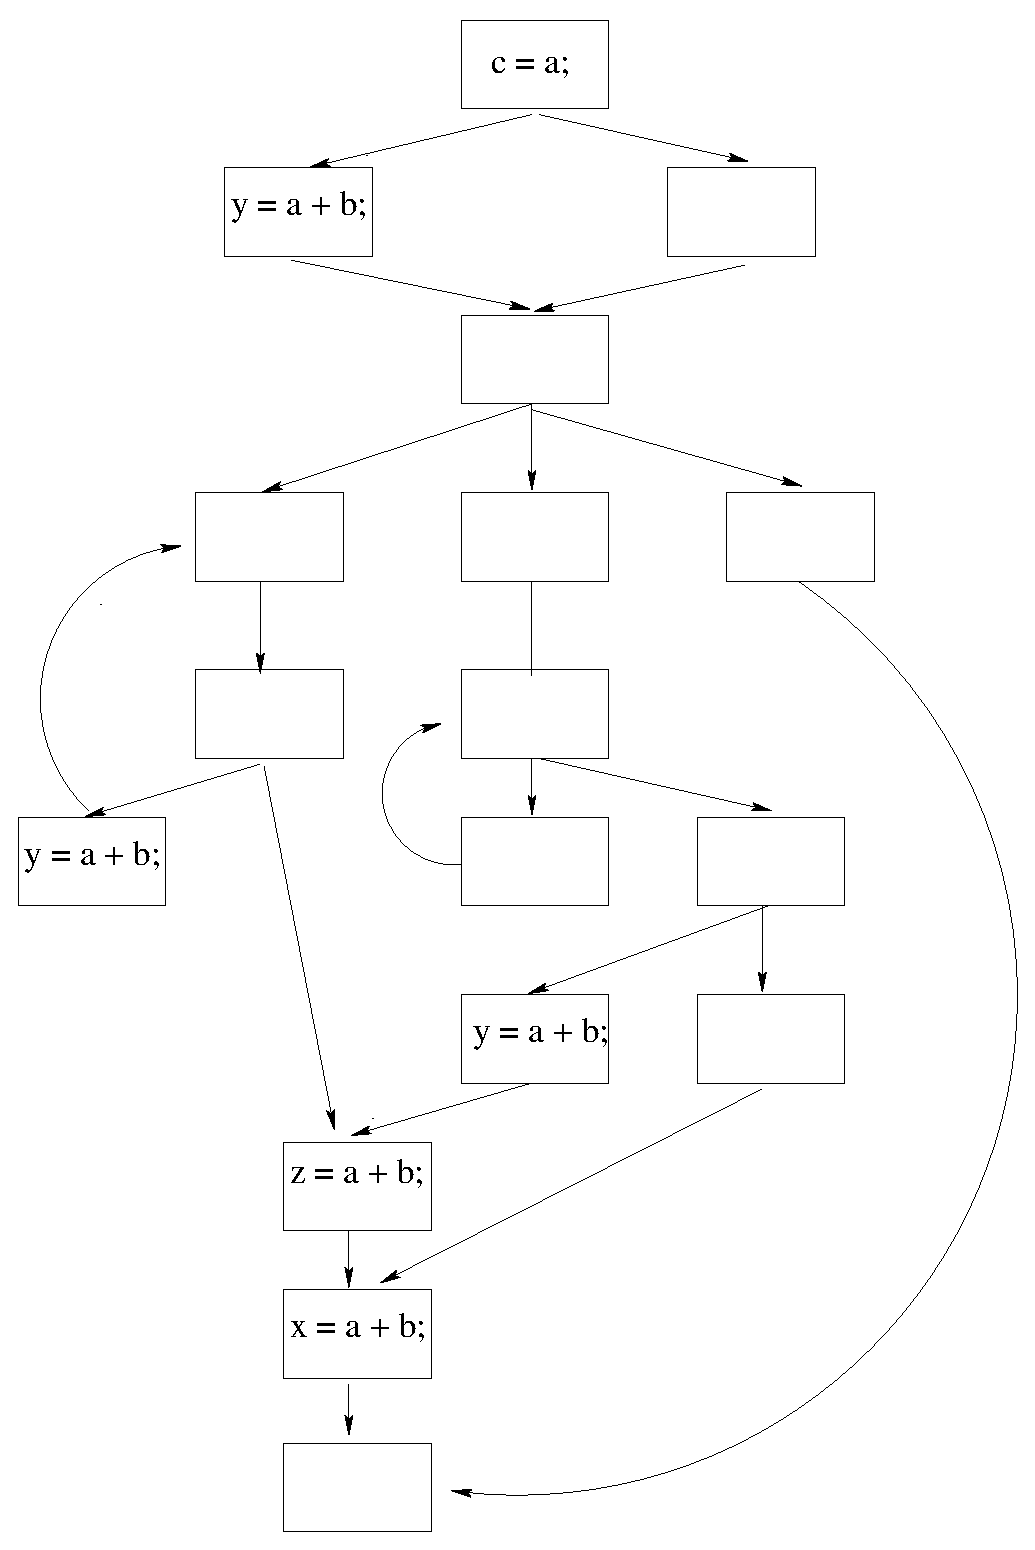
\includegraphics[scale=0.6]{3} & \includegraphics[scale=0.6]{4} \\
      &\\
  \text{The motivating example} &
  \text{Lazy code motion transformation as suggested by our implementation } \\
    \end{tabular}}
  \end{center}
  \caption{\label{fig:2} }
\end{figure}

\bibliography{CS526_project_proposal}

%\appendix

\chapter{Computation of localized sets}
For each basic block there are 3 bit vectors dedicated to the block-specific
properties, namely \texttt{Transp}, \texttt{Antloc} and \texttt{Xcomp}. As
mentioned before, a bit vector is a boolean array of value numbers.  Let the
leader expression (as defined in the section on value numbering) associated
with the value number $v$ be called $L(v)$. 


\begin{equation}
\begin{array}{l c l}
\texttt{Transp(v,B)} &=& \left\{
                    \begin{array}{l l}
                        false & \quad \text{iff $\exists$ x $\in$ operands of L(v) such that \texttt{Mod(x,B)} = true}\\
                        true & \quad \text{Otherwise}
                    \end{array} \right. \\
\texttt{Antloc(v,B)} &=& \texttt{Eval(v,B)} \cap \texttt{Transp(v,B)} \\
\texttt{Xcomp(v,B)} &=& \texttt{Eval(v,B)} \cap \overline{\texttt{Transp(v,B)}}\\
  &&\\
\text{where}&& \\  
\quad \texttt{Eval(v,B)} &=& \text{\{v $|$ value number v is computed in B\}}\\
\quad \texttt{Mod(op,B)} &=& \text{operand op modified in B}\\
\end{array}
\end{equation}

\chapter{Lazy Code motion Transformations}

\begin{itemize}
\item Down Safety Analysis (Backward data flow analysis)
\begin{equation}
\begin{array}{l c l}
\antin{b} &=& \antloc{b} \cup (\transp{b} \cap \antout{b}) \\
\antout{b} &=& \xcomp{b} \cup \left\{
                    \begin{array}{l l}
                        \phi & \quad \text{if b = exit}\\
                        \displaystyle \bigcap_{s \in succ(b)} \antin{s} &
                    \end{array} \right. \\
\end{array}
\end{equation}

\item Up Safety Analysis (Forward data flow analysis)
\begin{equation}
\begin{array}{l c l}
\availin{b} &=& \left\{
                  \begin{array}{l l}
                        \phi & \quad \text{if b = entry}\\
                        \displaystyle \bigcap_{p \in pred(b)} (\xcomp{p} \cup \availout{p}) & 
                  \end{array} 
              \right. \\
\availout{b} &=& \transp{b} \cap (\antloc{b} \cup \availin{b}) \\
\end{array}
\end{equation}

\item Earliest-ness (No data flow analysis)
\begin{equation}
\begin{array}{l c l}
\earlin{b}  &=& \antin{b} \cap \displaystyle \bigcap_{p \in pred(b)} (\overline{\availout{p} \cup \antout{p}}) \\ 
\earlout{b} &=& \antout{b} \cap \overline{\transp{b}}
\end{array}
\end{equation}

\item Delayability (Forward data flow analysis)
\begin{equation}
\begin{array}{l c l}
\delayin{b} &=& \earlin{b} \cup  \left\{
                              \begin{array}{l l}
                                \phi & \quad \text{if b = entry}\\
                                \displaystyle \bigcap_{p \in pred(b)} (\overline{\xcomp{p}} \cap \delayout{p}) & 
                  \end{array} 
              \right. \\
\delayout{b} &=& \earlout{b} \cup (\delayin{b} \cap \overline{\antloc{b}}) \\
\end{array}
\end{equation}

\item Latest-ness (No data flow analysis)
\begin{equation}
\begin{array}{l c l}
\latestin{b}  &=& \delayin{b} \cap \antloc{b}\\
\latestout{b} &=& \delayout{b} \cap (\xcomp{b} \cup \displaystyle \bigcup_{s \in succ(b)} \overline{\delayin{s}})
\end{array}
\end{equation}


\item Isolation Analysis (Backward data flow analysis)
\begin{equation}
\begin{array}{l c l}
\isoin{b} &=& \earlout{b} \cup \isoout{b} \\
\isoout{b} &=& \left\{
                    \begin{array}{l l}
                        U & \quad \text{if b = exit}\\
                        \displaystyle \bigcap_{s \in succ(b)} (\earlin{s} \cup (\overline{\antloc{s}} \cap \isoin{s}) )&
                    \end{array} \right. \\
\end{array}
\end{equation}

\item Insert and Replace points
\begin{equation}
\begin{array}{l c l}
\insertin{b} &=& \latestin{b} \cap \overline{\isoin{b}} \\
\insertout{b} &=& \latestout{b} \cap \overline{\isoout{b}} \\
&&\\
\replacein{b} &=& \antloc{b} \cap \overline{\latestin{b} \cap \isoin{b}} \\
\replaceout{b} &=& \xcomp{b} \cap \overline{\latestout{b} \cap \isoout{b}}
\end{array}
\end{equation}
\end{itemize}

\chapter{Generalized data flow framework}

All the equations in Appendix B can be computed using the generic
framework defined below.

\section{Forward Analysis}
\begin{equation}
\begin{array}{l c l}
\myin{b} &=& \Alpha{b} \cup  \left\{
                    \begin{array}{l l}
                        \bot & \quad \text{if b = entry}\\
                        \displaystyle \bigwedge_{p \in pred(b)} \Beta{p}&
                    \end{array} \right. \\
\myout{b} &=& \myGamma{b}                      
\end{array}
\end{equation}

\section{Backward Analysis}
\begin{equation}
\begin{array}{l c l}
\myin{b} &=& \myGamma{b}                      \\
\myout{b} &=& \Alpha{b} \cup  \left\{
                    \begin{array}{l l}
                        \bot & \quad \text{if b = exit}\\
                        \displaystyle \bigwedge_{s \in succ(b)} \Beta{s}&
                    \end{array} \right. \\
\end{array}
\end{equation}

The following is the function which we call with dataflow equation
specific parameters defined subsequently.

\begin{framed}
\[
\texttt{callFramework}(\myout{b}, \myin{b}, \Alpha{b}, \Beta{b},\myGamma{b}, \bigwedge, \bot, \top, \text{Direction})
\]
\end{framed}

Following is the list of values that we need to plug-in to $\alpha$,
          $\beta$ and $\gamma$ for the above generic framework
          to work.



\begin{itemize}
\item Down Safety Analysis (Backward data flow analysis)
\begin{equation}
\begin{array}{l c l}
\Alpha{x}     &=& \xcomp{x} \\
\Beta{x}      &=& \antin{x}     \\     
\myGamma{x}   &=& \transp{x} \cap \antout{x} \cup \antloc{x}\\
\bigwedge     &=&  \cap \\
\bot          &=& \phi \\
\top          &=& V, \text{set of all values} \\
\text{Direction}    &=& \text{Backward}
\end{array}
\end{equation}

\item Up Safety Analysis (Forward data flow analysis)
\begin{equation}
\begin{array}{l c l}
\Beta{x}      &=& \xcomp{x} \cup \availout{x}     \\     
\myGamma{x}   &=& \antloc{x} \cup \availin{x} \cap \transp{x}\\
\bigwedge     &=&  \cap \\
\bot          &=& \phi \\
\top          &=& V, \text{set of all values} \\
\text{Direction}    &=& \text{Forward}
\end{array}
\end{equation}

\item Delayability (Forward data flow analysis)
\begin{equation}
\begin{array}{l c l}
\Alpha{x}     &=& \earlin{x} \\
\Beta{x}      &=& \overline{\xcomp{x}} \cap \delayout{x}     \\     
\myGamma{x}   &=& \delayin{x} \cap \overline{\antloc{x}} \cup \earlout{x}\\
\bigwedge     &=&  \cap \\
\bot          &=& \phi \\
\top          &=& V, \text{set of all values} \\
\text{Direction}    &=& \text{Forward}
\end{array}
\end{equation}

\item Isolation Analysis (Backward data flow analysis)
\begin{equation}
\begin{array}{l c l}
\Beta{x}      &=& \overline{\antloc{x}} \cap \isoin{x} \cup \earlin{x}     \\     
\myGamma{x}   &=& \earlout{x} \cup \isoout{x} \\
\bigwedge     &=&  \cap \\
\bot          &=& V, \text{set of all values} \\
\top          &=& V, \text{set of all values} \\
\text{Direction}    &=& \text{Backward}
\end{array}
\end{equation}

\end{itemize}

\chapter{Transformations for ``Zero-trip Loops''}

\begin{figure}[htbp]
  \begin{center}
     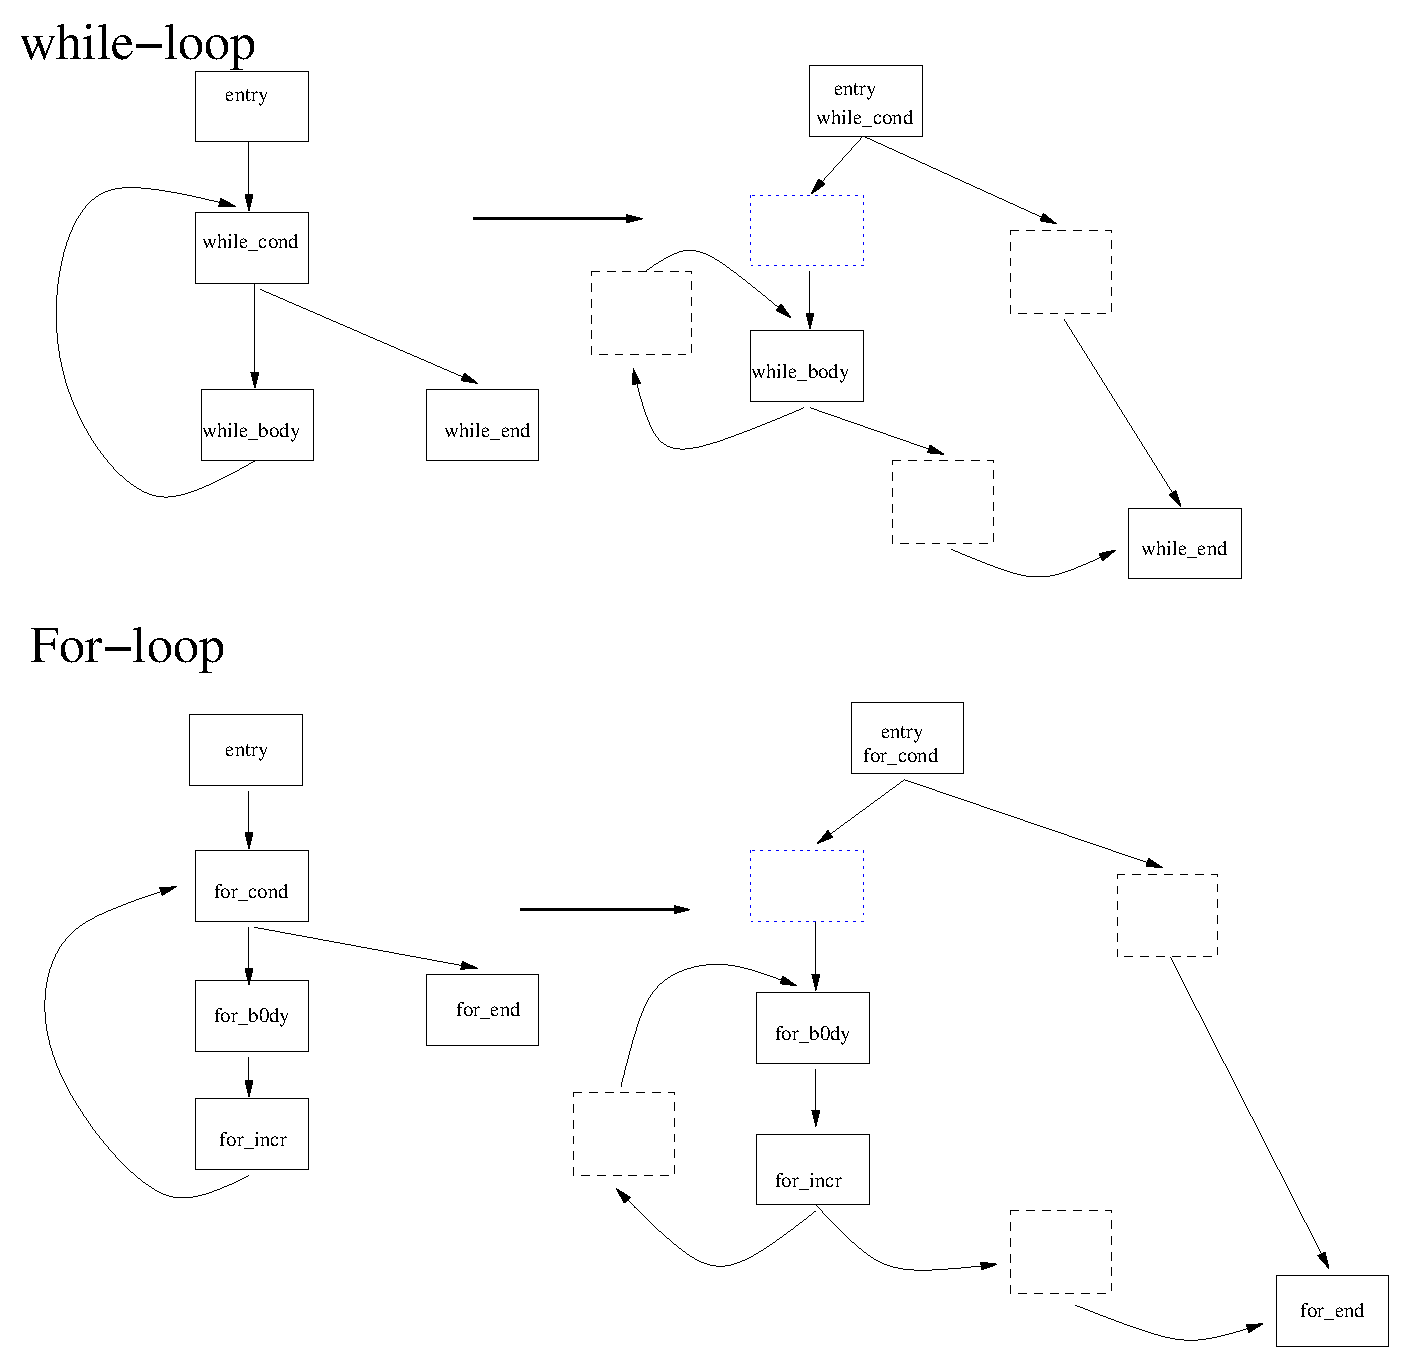
\includegraphics[scale=0.5]{Figs/5} 
  \end{center}
  \caption{Loop transformations done by \emph{-loop-rotate}. \emph{do-while}
    loops remain unaffected. Blue dotted boxes are the ones inserted by loop
      rotate. PRE can insert the computations in these places.}
  \label{fig:5} 
  \end{figure}


\chapter{An Extended Example}

Here we show, through an example code, the optimizations performed
by our PRE pass. The intention here is to highlight redundancy elimination for  
expressions $a + b$ \& $a < b$. Optimal placements are marked in Figure \ref{fig:2}.
Some of the notable obseravtions are:
\begin{itemize}
\item Black dotted boxes denote basic blocks inserted because of critical edge splitting
\item  Blue dotted boxes are the loop pre-headers inserted
      by -loop-rotate pass. PRE can insert computations here.
\item Inserted statements are marked \textcolor{blue}{blue} and replaced ones with
      \textcolor{magenta}{magenta}      
\item LCSE (Local common subexpression elimination)  happened in BB2.
\item For the loop {BB7,BB9} in Figure \ref{fig:1}, LICM happened wherein the computation 
of $a+b$ is moved from BB9 (in Figure  \ref{fig:1}) to BB8 (in Figure \ref{fig:2}). BB8 is the loop pre-header
\end{itemize}


\begin{figure}[htbp]
  \begin{center}
     \includegraphics[scale=0.3]{Figs/1} 
  \end{center}
  \caption{A motivating example}
    \label{fig:1} 
\end{figure}

\begin{figure}[htbp]
  \begin{center}
     \includegraphics[scale=0.3]{Figs/2} 
  \end{center}
  \caption{Lazy code motion transformation on computations $a + b$ \& $a < b$.}
  \label{fig:2} 
\end{figure}


%\nocite{*}


\end{document}
